\apendice{Documentación de usuario}

\section{Introducción}

En este anexo se indicarán los distintos requisitos necesarios para ejecutar las diversas aplicaciones desarrolladas durante el proyecto. Así como, toda la información necesaria para la correcta utilización de la herramienta. Y la solución ante posibles problemas en su utilización.

\section{Requisitos de usuarios e instalación}

Los requisitos \textit{software} necesarios para poder ejecutar las aplicaciones son:

\begin{itemize}
	\item Anaconda. Descargando e instalando la versión para Python 3.6\footnote{Es altamente recomendable utilizar \textit{Anaconda} para la instalación de \textit{Python} junto a algunos paquetes necesarios. Puesto que la instalación aislada de \textit{Python} llevaría al usuario a tener que instalar manualmente múltiples paquetes que ya vienen preinstálados con \textit{Anaconda}.}.

	\item IPython File Upload. Siguiendo los pasos de instalación en \url{https://github.com/peteut/ipython-file-upload}.

	\item \textit{Jupyter Dashboards}. Siguiendo los pasos de instalación en \url{https://github.com/jupyter/dashboards}.

	\item Este proyecto se puede descargar o clonar desde el siguiente enlace al repositorio: \url{https://github.com/jasag/Phytoliths-recognition-system}. Entrando, preferiblemente, en la pestaña de \textit{Releases} y descargando el zip \textit{v0.1.0}. Véase la figura \ref{fig:E.4.0}.

\end{itemize}

\begin{figure}[h]
\centering
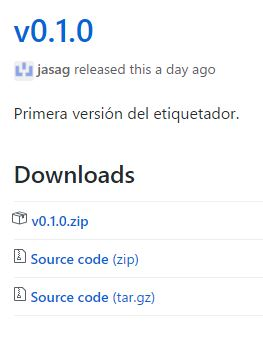
\includegraphics[width=0.40\textwidth]{v010}
\caption{Primera versión del etiquetador}
\label{fig:E.4.0}
\end{figure}

\section{Manual del usuario}

En esta sección se explicarán los distintos aspectos a tener en cuenta en el uso de los distintos productos.

\subsection{Manual del usuario: etiquetador de imágenes}

Una vez completados satisfactoriamente los pasos anteriores,  ejecutamos \textit{Jupyter Notebook} desde \textit{Anaconda}\footnote{ Si es la primera vez que utilizas Anaconda es recomendable utilizar Anaconda Navigator. Ya que este nos facilitará ejecutar \textit{Jupyter Notebook}, sin el uso de la linea comandos.}. Y desde esta aplicación, abrimos el \textit{notebook} \textit{Image\_Labeler.ipynb}, en la carpeta \textit{code/notebooks} dentro de este proyecto previamente descargado.

Con \textit{Image\_Labeler.ipynb} ya abierto, tendremos que navegar por la barra de navegación del \textit{notebook} para llevar a cabo los dos siguientes pasos:

\begin{enumerate}[1.]
    \item Ejecutar todas las celdas del \textit{notebook}.  Para ello, navegamos por \textit{Cell} y clicamos en \textit{Run All}. Como se puede observar en la figura \ref{fig:E.4.1}.
    \item Activar \textit{Dashboard Preview}. Para ello, navegamos por \textit{View} y clicamos en \textit{Dashboard Preview} \ref{fig:E.4.2}.
\end{enumerate}

\begin{figure}[h]
\centering
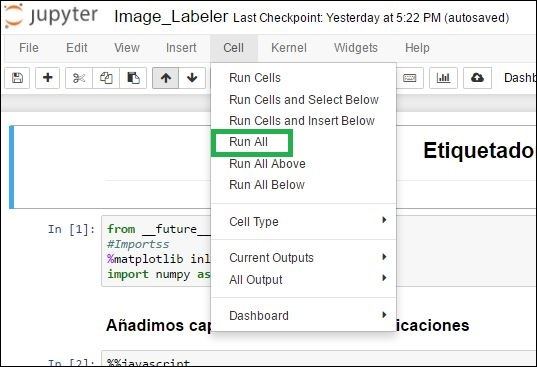
\includegraphics[width=0.80\textwidth]{ejecucion_todas_las_celdas}
\caption{Ejecución de todos los pasos del \textit{notebook}}
\label{fig:E.4.1}
\end{figure}

\begin{figure}[h]
\centering
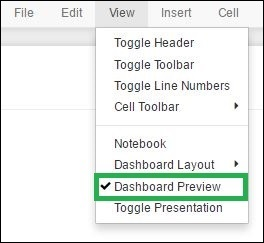
\includegraphics[width=0.60\textwidth]{cambio_de_vista_a_preview_dashboard}
\caption{Selección de la vista del \textit{notebook}}
\label{fig:E.4.2}
\end{figure}

Una vez realizados los pasos anteriores, tendremos como resultado la pantalla inicial del etiquetador, tal y como se observa en la figura \ref{fig:E.4.3}.

\begin{figure}[h]
\centering
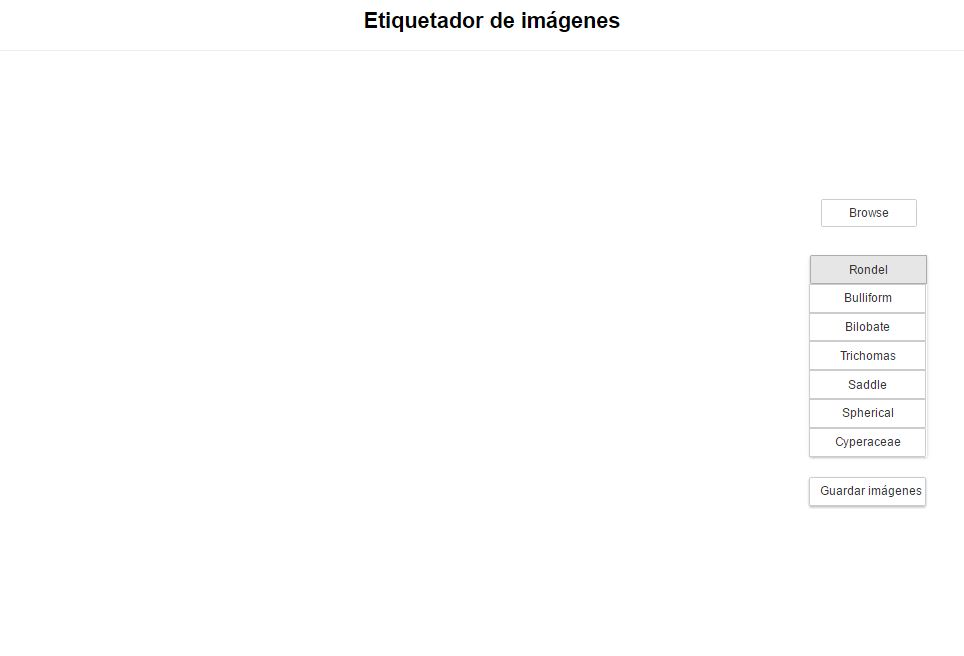
\includegraphics[width=0.99\textwidth]{etiquetador_de_imagenes_antes_de_cargar_imagen_v1}
\caption{Etiquetador de imágenes}
\label{fig:E.4.3}
\end{figure}

\subsubsection{Uso del etiquetador}

Como resultado de los pasos previos, el etiquetador de imágenes estará listo para su funcionamiento. 

El etiquetador está compuesto por dos partes principales:

\begin{itemize}
	\item Parte izquierda: imagen donde etiquetar los fitolitos.
	\item Parte derecha: \textrm{<<botones>>}.	
\end{itemize}

La parte izquierda mostrará la imagen a ser etiquetada. Y la parte derecha mostrará los botones que nos permitirán seleccionar los distintos tipos de fitolitos presentes en la imagen. Como podemos ver en la figura \ref{fig:E.4.3}.

\subsubsection{Parte derecha del etiquetador: botonera}
La parte derecha del etiquetador esta compuesta por tres grupos de botones. El botón para la carga de una imagen, los botones de selección de fitolito y el botón de guardado. Como podemos obsevar en la figura \ref{fig:E.4.7}. En las secciones siguientes explicaré sus funciones. 

\begin{figure}[h]
\centering
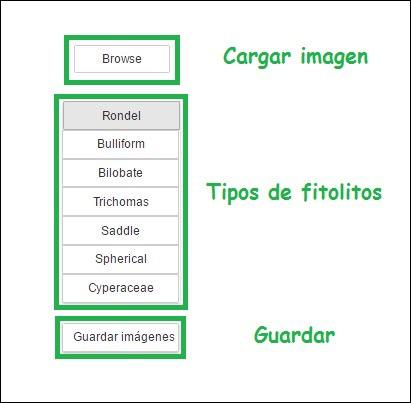
\includegraphics[width=0.50\textwidth]{etiquetador_botones}
\caption{Parte derecha del etiquetador}
\label{fig:E.4.7}
\end{figure}

\subsubsection{Cargar imagen}

Para etiquetar una imagen, el primer paso será escoger una imagen en nuestro ordenador mediante el botón \textit{Browse}, situado en la esquina superior derecha del etiquetador. Como se puede ver en la figura \ref{fig:E.4.3}.

Una vez  pulsado, se mostrará una ventana, véase figura \ref{fig:E.4.4}, en la que escogeremos la imagen que deseemos.

\begin{figure}[h]
\centering
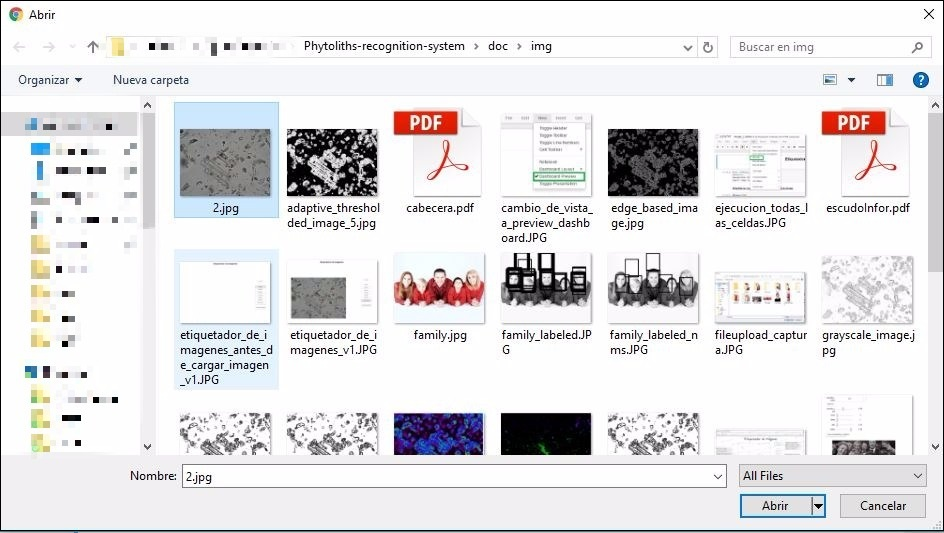
\includegraphics[width=0.99\textwidth]{fileupload_captura}
\caption{Ventana de subida de ficheros}
\label{fig:E.4.4}
\end{figure}

Tras escoger la imagen, esta se cargará en la parte izquierda del etiquetador, dando lugar a algo similar a lo mostrado en la figura \ref{fig:E.4.5}.

\begin{figure}[h]
\centering
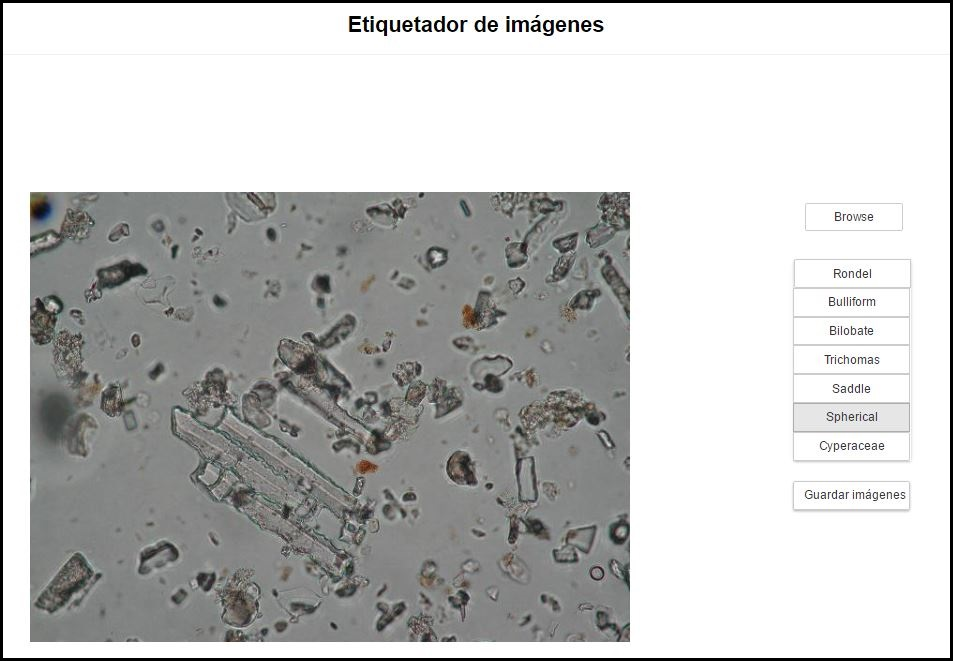
\includegraphics[width=0.99\textwidth]{etiquetador_de_imagenes_2_v1}
\caption{Etiquetador de imágenes con una imagen cargada}
\label{fig:E.4.5}
\end{figure}

\subsubsection{Etiquetar distintos tipos de fitolitos}
Antes de explicar como se crean las etiquetas, debemos de tener en cuenta los botones para la selección de tipos de fitolito.

Cada vez que se quiera etiquetar un tipo de fitolito distinto tendremos que pulsar en el botón correspondiente al tipo de fitolito objetivo.

A su vez, y para facilitarnos distinguir a que tipo de fitolito pertenece cada etiqueta, se escribe encima de cada etiqueta el tipo de fitolito que ha sido etiquetado, véase figura \ref{fig:E.4.6}.

\begin{figure}[h]
\centering
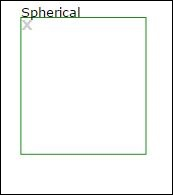
\includegraphics[width=0.30\textwidth]{etiqueta_ejemplo}
\caption{Ejemplo de etiqueta}
\label{fig:E.4.6}
\end{figure}

\subsubsection{Realizar etiquetas}

Una vez cargada la imagen en el etiquetador, y comprendido el uso de los botones de selección de tipo de fitolito, podemos comenzar a  etiquetar fitolitos. Para etiquetar, basta con clicar en la imagen, definiendo una esquina del rectangulo, mover el ratón hacía donde deseemos y volver a clicar, definiendo la otra esquina de este. Para, así, definir una etiqueta como la que se puede ver en la figura \ref{fig:E.4.6}.

\subsubsection{Eliminar etiquetas}

Como es normal, un usuario puede equivocarse dibujando una etiqueta que no deseaba. Por ello, en la esquina superior izquierda de cada etiqueta, disponemos de una \textrm{<<X>>}, como se observa en la figura \ref{fig:E.4.6}, que nos permitirá eliminar etiquetas previamente realizadas. Posibilitando así revertir un error del usuario.

\subsubsection{Guardar etiquetas}

Después de realizar todas las etiquetas, tan solo queda guardarlas. Para ello basta con clicar el botón \textrm{<<Guardar imágenes>>} en la esquina inferior derecha del etiquetador, véase la figura \ref{fig:E.4.3}.

Es \textbf{importante} destacar que no sirve de nada etiquetar una imagen, si no pulsamos más tarde en el botón guardar. Debido a que las etiquetas realizadas no habrán sido guardadas. Y, por lo tanto, todas las etiquetas realizadas sobre una imagen se perderán.

\subsubsection{Etiquetas realizadas fuera de la imagen}

En la versión actual del etiquetador, este te permite realizar etiquetas fuera de la imagen. Pero estas etiquetas no serán guardadas.

Por lo tanto, debemos de tener en cuenta que las etiquetas que no tengan todas sus aristas dentro de la imagen no se guardan.

Aun así, en la siguiente sección explicaré como comprobar que las etiquetas previamente realizadas han sido guardadas.

\subsubsection{Carga de etiquetas previamente realizadas}

Las imágenes etiquetadas se guardan en la carpeta \textit{/code/rsc/img} dentro de la carpeta contenedora del proyecto. Al cargar imágenes que se encuentren dentro de esta carpeta, las etiquetas previamente realizadas sobre estas imágenes se cargarán con ellas\footnote{Nótese que los nombres de las imágenes no son los cargados originalmente, ya que todas las imágenes etiquetadas son renombradas para no sobrescribir imágenes previamente etiquetadas con nombres iguales.}. Esto nos permitirá poder añadir nuevas etiquetas a imágenes ya procesadas, modificarlas o eliminarlas.

\subsubsection{Notificaciones}

Se han incluido en el etiquetador una serie de notificaciones, las cuales nos permitirán cercionarnos de distintos eventos. Las notificaciones que se muestran son las siguientes:

\begin{enumerate}
	\item Notificación en la carga de una imagen. Véase la figura \ref{fig:E.4.8.1}.
	\item Notificación en la carga incorrecta de un fichero que no sea una imagen. Véase la figura \ref{fig:E.4.8.2}.
	\item Notificación en el guardado de etiquetas. Véase la figura \ref{fig:E.4.8.3}.
\end{enumerate}

Gracias a estas notificaciones podremos saber si la imagen que hemos seleccionado era correcta, o no, y si las etiquetas ya han sido guardadas.

\begin{figure}[h]
\centering

\includegraphics[width=0.60\textwidth]{notificacion_carga_de_imagen_correctamente}
\caption{Notificación en la carga de una imagen}
\label{fig:E.4.8.1}
\end{figure}

\begin{figure}[h]
\centering

\includegraphics[width=0.70\textwidth]{notificacion_carga_de_imagen_incorrectamente}
\caption{Notificación en la carga incorrecta de un fichero que no sea una imagen}
\label{fig:E.4.8.2}
\end{figure}

\begin{figure}[h]
\centering

\includegraphics[width=0.70\textwidth]{notificacion_guardado_correctamente}
\caption{Notificación en el guardado de etiquetas}
\label{fig:E.4.8.3}
\end{figure}

\subsubsection{Bloqueo del etiquetador}

En algunas ocasiones, y por razones que desconozco hasta el momento, el etiquetador puede bloquearse al cargar imágenes previamente etiquetadas. Para solucionar este problema, basta con recargar el etiquetador, yendo a la barra de navegación, navegando por \textit{Cell} y finalmente clicando en \textit{Run All}. Como hicimos en la puesta en marcha del etiquetador.